\documentclass{article}
\usepackage[utf8]{inputenc}
\usepackage[left=1in,top=1in,right=1in,bottom=1in,bindingoffset=0cm]{geometry}
\usepackage{commath, amsmath,amssymb,amsthm,mathtools,mathrsfs}
\usepackage[spanish]{babel}
\usepackage{setspace}
\usepackage{footnote}
\usepackage{minipage-marginpar}
\usepackage{dashbox}
\usepackage{dsfont}
\usepackage{hyperref}
\usepackage{bm}
\usepackage{indentfirst}
\usepackage{titlesec}
\usepackage{csquotes}
\usepackage{minipage-marginpar}
\usepackage{multicol}
\usepackage[shortlabels]{enumitem}
\usepackage[backend=biber]{biblatex}
\addbibresource{bibliography.bib}




% COMMANDS
\newcommand{\HRule}{\rule{\linewidth}{0.5mm}}


\begin{document}
    


\begin{titlepage}
    \begin{center}
    
\includegraphics[width=0.25\textwidth]{resources/unam_escudo.png}~\\[2cm]
    \textsc{\huge Universidad Nacional Autónoma de México}\\[0.5cm]  
    \textsc{\LARGE Instituto de Matemáticas}\\[2cm]
    
    \HRule \\[0.5cm] 
    {\Huge \bfseries Interpretabilidad de los \\[1cm] Ataques Adversarios} \\[0.3cm] 
    \HRule \\[0.5cm]
    
    \textsc{\LARGE Reporte del Proyecto Final}\\[0.4cm]
    \textsc{\LARGE - Redes Neuronales - }\\[3cm]
    
    % Authors 

    {\Large
    \begin{tabular}{ccc}
        Aaron Kelley & \hspace{1.5in} & Rodrigo Fritz
    \end{tabular}
    }
    % {\Large \hspace{0.5in} \& Aaron Kelley\hspace{1.5in} }
    \vfill

    % Bottom of the page  
    {\Large 18 de junio, 2021}
    
    \end{center} 
\end{titlepage}
Abstract Goes here \\[1cm]

\noindent\textbf{Keywords}:  
\tableofcontents
\vspace{1in}
{\Large \noindent Development Notes/Ideas}
\begin{itemize}
    \item maybe we should take out Projected Gradient Descent
    \item with cleverhans we can do targeted attacks with Fast Gradient Descent
\end{itemize}
\pagebreak
\section{Introducción}

Las redes neuronales profundas (DNNs) han ganado una alta reputación con respecto a sus capacidades de clasificar imágenes con tanta precisión (y en algunos casos con una precisión incluso superior) como la de los humanos. Pero es cada vez más claro que las redes aprenden a clasificar de una manera muy distinta a la de los humanos. Una de las propiedades que demostró eso fue el descubrimiento de su susceptibilidad a los ataques adversarios \cite{szegedy2014intriguing}. Estos ataques se construyen agregándoles a las imágenes una pequeña perturbación, imperceptible para los humanos, pero que engaña a la red, es decir, aunque una imagen adversaria para nosotros parezca igual a la original, la red tiene una alta probabilidad de clasificar mal a la imagen adversaria. Dado que los ataques, en general, no son detectables por los humanos, se plantea la preocupación de que puedan ser usados maliciosamente; por ejemplo, en la tecnología de reconocimiento de imágenes que se utiliza en los automóviles autónomos, por eso se requiere más profundizar en el conocimiento asociado a estos ataques adversarios.

A grandes rasgos, los ataques pueden dividirse en dos categorías: dirigidos y no dirigidos. El objetivo de los ataques no dirigidos es que cambien la clasificación correcta por cualquier otra, mientras que los ataques dirigidos buscan cambiar la clasificación correcta por una clasificación específica. En el caso de los ataques no dirigidos, generalmente se usa el gradiente de manera directa: se toma el gradiente de la función de pérdida con respecto a la imagen y eso se usa para diseñar una perturbación que maximice el error de la clasificación cuando se le agrega a la imagen. Dos ejemplos de ataques no dirigidos que utilizan el gradiente directamente son el \textbf{projected gradient descent} (PGD) \cite{madry2019deep} y el \textbf{fast gradient sign method} (FGSM) \cite{goodfellow2015explaining}. Este último toma el signo de cada elemento del gradiente en lugar de usar el valor del gradiente, esto hace que sea más rápido con grandes cantidades de datos. En este trabajo utilizamos el \textbf{fast gradient method} FGM (con norma $L_2$), el FGSM (FGM con norma $L_\infty$) y el ataque con norma $L_2$ de Carlini y Wagner (CW) para explorar los ataques no-dirigidos. El ataque de Carlini y Wager puede ser dirigido o no-dirigido. 

Cabe mencionar la diferencia entre los ataques de caja blanca y caja negra. En el primero, todos los detalles de la red (pesos, arquitectura, etc.) son conocidos por el atacante. Por el contrario, en los ataques de caja blanca, los detalles están escondidos, y solo se conocen las entradas (inputs) y las salidas (outputs). Aunque parezca muy difícil, los ataques de caja negra son bastante exitosos por la facilidad de aproximar el gradiente solo por las entradas y las salidas. Los ataques que se emplean en este artículo son los de caja blanca.

Desde el descubrimiento de la vulnerabilidad que tienen las DNNs ante los ataques adversarios, se han diseñado defensas para tratar de combatir los ataques. Aunque ninguna defensa funciona para resistir completamente los ataques, muchas sí tienen efecto, y vale la pena explorar qué propiedades contribuyen a su éxito. Al igual que los ataques, las defensas también se pueden categorizar en dos modalidades. Las del primer tipo modifican el entrenamiento de la red para que la función de pérdida se vuelva más suave. Entre más suave sea esa función, más difícil será que las perturbaciones pequeñas hagan grandes cambios. Un ejemplo conocido de este tipo es el entrenamiento adversario \cite{goodfellow2015explaining, Shaham_2018, szegedy2014intriguing}. Las defensas del segundo tipo no modifican el entrenamiento ni la arquitectura, sino que utilizan un preprocesamiento en las imágenes de entrada. La defensa que se utiliza en este artículo corresponde al segundo tipo y es la compresión JPEG \cite{das2017keeping}.

En este trabajo estudiamos la eficacia de la compresión JPEG en contra de los ataques y estudiamos el efecto que tienen el overfitting y la overparameterization en las redes y, dado que nuestro objetivo fue encontrar una medida de interpretabilidad de los ataques adversarios, empleamos análisis de frecuencias para observar si las redes funcionan como un filtro en el sentido de teoría de control, específicamente esperando encontrar un comportamiento del tipo pasabandas, ya que esa es más o menos la manera en que nuestra mente clasifica imágenes, y analizamos la prominencia (saliency) \cite{simonyan2014deep} de las imágenes para saber cuáles son las regiones en las que las redes se enfocan cuando analizan las imágenes.
\pagebreak
\section{Método}

\subsection{Datos}
Para entrenar nuestras redes y probar los ataques adversarios y las defensas contra ellos, se emplearon las dos bases de datos más sencillas para procesamiento de imágenes: MNIST y CIFAR-10.

\subsubsection{MNIST}
La base de datos MNIST es un compendio de los dígitos del 0 al 9 en letra manuscrita con 60,000 imágenes para entrenar a distintos sistemas de procesamiento de imágenes y 10,000 imágenes para evaluarlos. Se trata de un subconjunto de imágenes de un conjunto más grande que compiló el National Institute of Standards and Technology (NIST) del Departamento de Comercio los EEUU. Las siglas MNIST database significan Modified NIST database. Es una buena base de datos para probar técnicas de aprendizaje y métodos de reconocimiento de patrones con datos del mundo real empleando un esfuerzo mínimo en preprocesamiento y formato.

De las 10,000 imágenes de evaluación, la mitad fueron escritas por estudiantes de preparatoria y la otra mitad por empleados de la oficina de censos, mientras que de las 60,000 imágenes de entrenamiento, 58,527 de los números fueron escritos por 500 estudiantes y el resto por los empleados.

El tamaño de estas imágenes en blanco y negro fue normalizado a una caja de 20$\times$20 pixeles y se colocó su centro de masa en un campo de 28$\times$28 \cite{lecun2010mnist}. En la Figura \ref{mnist} se muestran algunos ejemplos de estas imágenes.

\begin{figure}[h]
    \centering
    \begin{subfigure}[b]{0.4\textwidth}
        \centering
        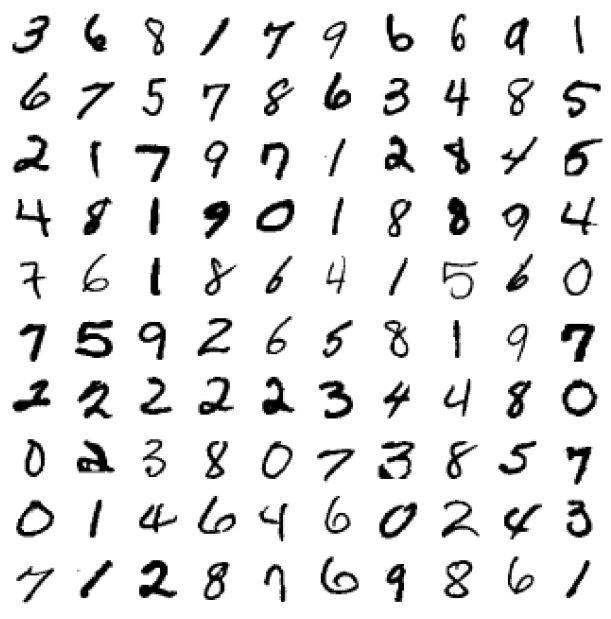
\includegraphics[width=\textwidth]{images/MNIST.png}
        \caption{Algunas imágenes del conjunto de evaluación de la base de datos MNIST \cite{Lecun98}.}
        \label{mnist1}
    \end{subfigure}
    \hspace{1cm}
    \begin{subfigure}[b]{0.45\textwidth}
        \centering
        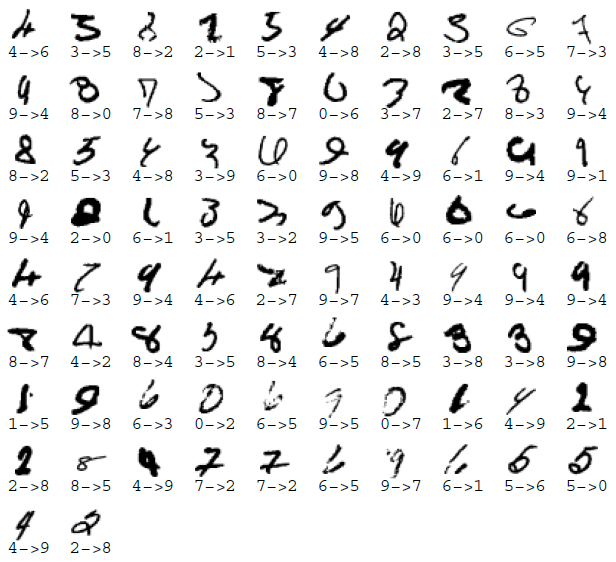
\includegraphics[width=\textwidth]{images/MNISTmiscl.png}
        \caption{82 imágenes de evaluación que LeNet-5 clasificó erróneamente \cite{Lecun98}.}
        \label{mnist2}
    \end{subfigure}
    \caption{Imágenes de MNIST.}
    \label{mnist}
\end{figure}

\subsubsection{CIFAR-10}
Los grupos del MIT y la NYU recopilaron un conjunto de millones de diminutas imágenes en color de la web, se trata de un excelente conjunto de datos para el entrenamiento no supervisado de modelos generativos profundos. Se crearon dos juegos de etiquetas confiables: el conjunto CIFAR-10, que tiene 6000 ejemplos de cada una de 10 clases y el conjunto CIFAR-100, que tiene 600 ejemplos de cada una de 100 clases que no se superponen. Usando estas etiquetas, se mostró que el reconocimiento de objetos mejora significativamente al entrenar previamente una capa de características en un gran conjunto de imágenes diminutas sin etiquetar.

Esta base de datos fue ensamblada buscando en la web imágenes de cada sustantivo en inglés no abstracto en la base de datos léxica WordNet. Utilizaron varios motores de búsqueda, incluidos Google, Flickr y Altavista y mantuvieron aproximadamente los primeros 3000 resultados para cada término de búsqueda. Después de recopilar todas las imágenes para un término de búsqueda en particular, eliminaron duplicados perfectos e imágenes en las que una parte excesivamente grande de los píxeles eran blancos, ya que tendían a ser figuras sintéticas en lugar de imágenes naturales. El término de búsqueda utilizado para encontrar una imagen le proporciona una etiqueta aproximada, aunque es extremadamente poco confiable debido a la naturaleza de la tecnología de búsqueda de imágenes en línea. En total, el conjunto de datos contiene 80 millones de imágenes en color reducidas a 32×32 y distribuidas en 79,000 términos de búsqueda \cite{Krizhevsky09learningmultiple}.

\begin{figure}[h!]
    \centering
    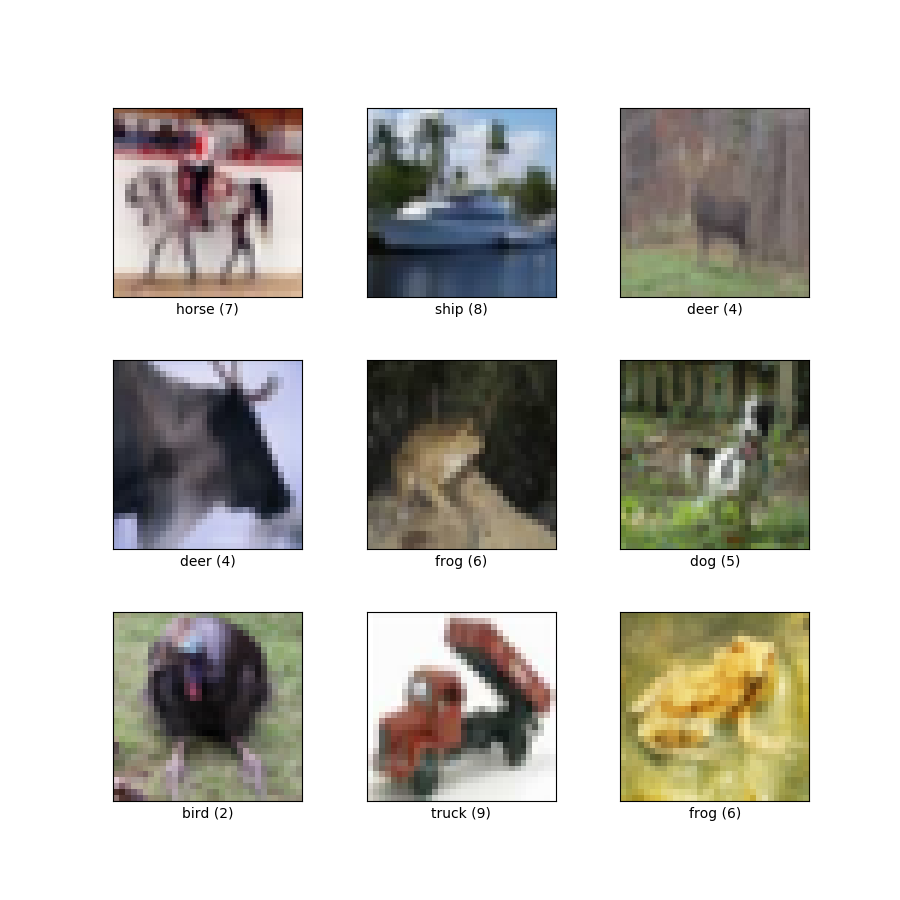
\includegraphics[width=0.71\textwidth]{images/cifar10-3.0.2.png}
    \caption{Algunas imágenes del conjunto de CIFAR-10 \cite{Krizhevsky09learningmultiple}}
    \label{cifar}
\end{figure}

El conjunto de datos se divide en cinco lotes de entrenamiento y un lote de prueba, cada uno con 10,000 imágenes. El lote de prueba contiene exactamente 1000 imágenes seleccionadas al azar de cada clase. Los lotes de entrenamiento contienen las imágenes restantes en orden aleatorio, pero algunos lotes de entrenamiento pueden contener más imágenes de una clase que de otra. Entre ellos, los lotes de entrenamiento contienen exactamente 5000 imágenes de cada clase \cite{cifarsite}. Las clases son:
\begin{multicols}{5}
\begin{enumerate}
    \item airplane
    \item automobile
    \item bird
    \item cat
    \item deer
    \item dog
    \item frog
    \item horse
    \item ship
    \item truck
\end{enumerate}
\end{multicols}


\subsection{Ataques}

\subsubsection{Fast Gradient Method}
\cite{goodfellow2015explaining, maybe more}

Sean $\theta$ los parámetros de un modelo, $x$ la entrada, $y$ las salidas asociadas, y $J(\theta, x, y)$ la función de costo. La función de costo se lineariza alrededor del valor actual de $\theta$. Sea $\epsilon \in \mathbb{R}^+$. Definamos la imagen adversaria 
\[\tilde{x} = x + \epsilon \eta_{\text{opt}}\]
Se puede definir $\eta_{\text{opt}}$ por el problema de optimización
\[\eta_{\text{opt}} = \operatornamewithlimits{argmax}_{\eta}\left\{ \operatorname{grad} ^\top \eta: \norm{\eta}_p< \epsilon\right\}\]
Donde $p \in \mathbb{N} \cup \{\infty\}$ y $\operatorname{grad} = \nabla_x J(\theta, x, y)$. Experimentamos con tres valores de $p$:
\begin{enumerate}[a)]
    \item $p = 1$, no lo sé, pero se encuentra en el codigo
    \item $p = 2$,
    \[\eta_{\text{opt}} = \frac{\operatorname{grad}}{\norm{\operatorname{grad}}}\]
    \item $p = \infty$,
    \[\eta_{\text{opt}} = \operatorname{sign}(\nabla_x J(\theta, x, y))\]
\end{enumerate}

\subsubsection{Carlini \& Wagner}
\cite{carlini2017evaluating} 

\subsection{Defensas}

\subsubsection{Compresión JPEG }
\cite{das2017keeping}
\pagebreak
\section{Resultados}
\subsection{Función Transferencia de las Redes}
Una manera útil de pensar de una red es con un punto de vista basado en teoría de control. De esta forma, construimos una función de transferencia calculando la respuesta de la red a ciertas frecuencias. 
\begin{figure}[h!]
    \centering
    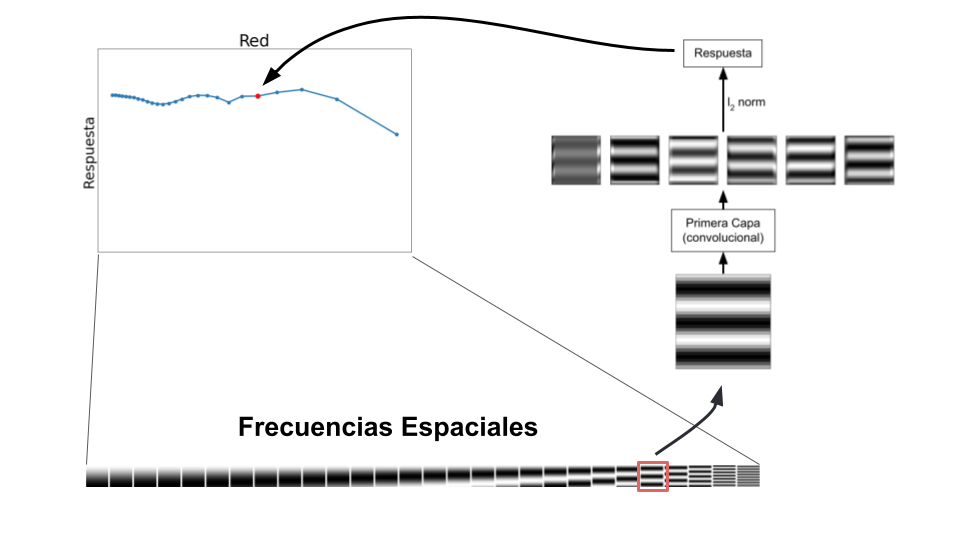
\includegraphics[width=\textwidth]{images/bode_diagrams/explanation_bode.png}
    \caption{stuff}
    \label{bode_explain}
\end{figure}

Así se puede ver las frecuencias a las que la red tiene mayor o menor sensibilidad.

\begin{figure}[h!]
    \centering
    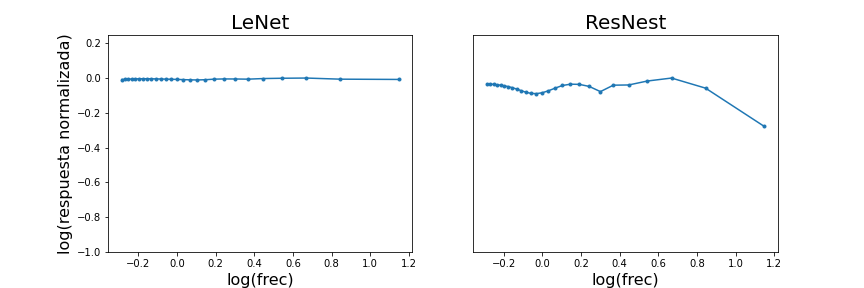
\includegraphics[width=\textwidth]{images/bode_diagrams/mnist_nets.png}
\end{figure}
\subsection{¿Qué hace la defensa de JPEG?}

Como vimos en la sección de compresión JPEG, cuando esta es aplicada a una imagen que ha sido sometida a un ataque adversario, los componentes de alta frecuencia se eliminan y, así como los humanos percibimos en menor medida dichos componentes, es posible que la red no logre distinguir el ataque perpetrado sobre la imagen, esto debido a que los ataques suelen tratarse de pequeñas cantidades de ruido o distorsión introducidos en la imagen y, al reducir la calidad de la misma, la red tiene más probabilidades de recuperar la clasificación original de la imagen. Esto se encuentra esquematizado en la Figura \ref{jpegexample}.

\begin{figure}[h!]
    \centering
    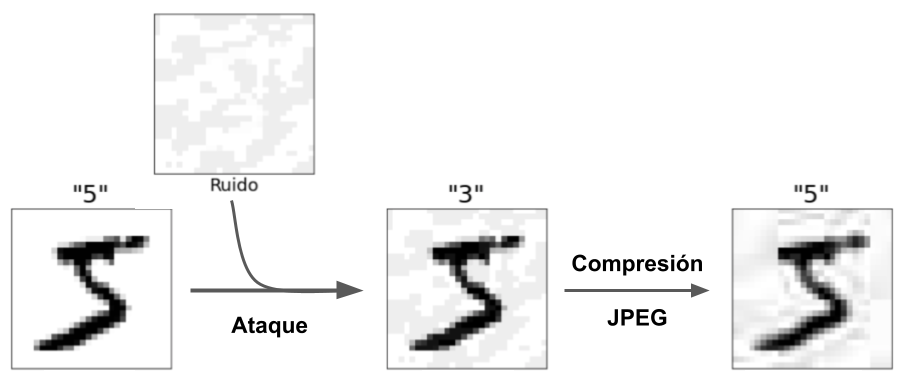
\includegraphics[width=0.8\textwidth]{images/jpeg/jpegdefense_example.png}
    \caption{La defensa JPEG radica en contrarrestar el ruido agregado por el ataque adversario al remover los componentes de alta frecuencia, que son los causantes de la falla en la clasificación de la red. En este ejemplo, el dígito 5 es clasificado como un 3 con el ruido del ataque, pero al hacer una compresión JPEG, la red clasifica correctamente al dígito como un 5.}
    \label{jpegexample}
\end{figure}

En la Figura \ref{jpeg_def} se muestra el resultado de nuestro entrenamiento de las redes LeNet y ResNet utilizando MNIST y el ataque FGSM con la norma $L_\infty$ para distintos niveles de compresión JPEG como defensa. Se observa que, efectivamente, conforme aumenta la compresión (disminuye la calidad), la precisión (accuracy) en la clasificación de las imágenes por parte de la red es mayor. Nótese que con ResNet la precisión decae más rápidamente conforme aumenta el épsilon.
\begin{figure}[h!]
    \centering
    \begin{subfigure}[b]{0.49\textwidth}
        \centering
        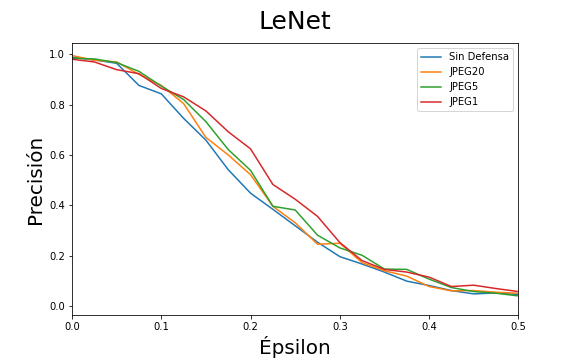
\includegraphics[width=\textwidth]{images/jpeg/jpegdefense_vs_epsilon_linear.png}
        \caption{Compresión JPEG contra FGSM usando LeNet}
    \end{subfigure}
    \begin{subfigure}[b]{0.49\textwidth}
        \centering
        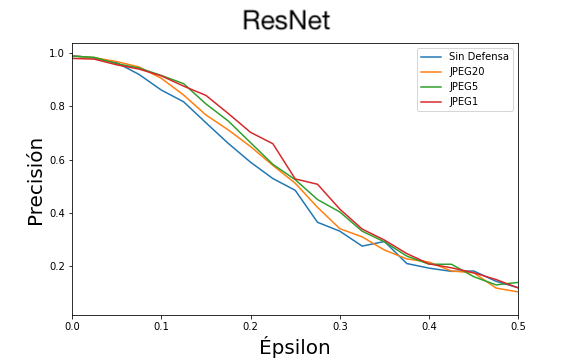
\includegraphics[width=\textwidth]{images/jpeg/jpegdefense_vs_epsilon_nonlinear.png}
        \caption{Compresión JPEG contra FGSM usando ResNet}
    \end{subfigure}
    \caption{Resultado de la compresión JPEG como defensa ante el ataque FGSM sobre MNIST}
    \label{jpeg_def}
\end{figure}
\pagebreak

\includemedia{images/bode_diagrams/resnet.swf}

{\LARGE \textbf{to do:}}
\begin{itemize}
    \item Carlini Wagner attack graphs
    \item JPEG defense graphs with cifar10
    \item Bode diagrams with jpeg conversion as first layer
    
    
\end{itemize}


% \begin{subfigure}[t]{0.22\textwidth}
% \centering
%     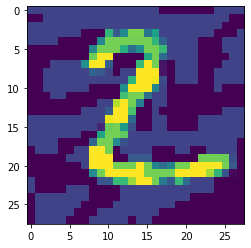
\includegraphics[width=\textwidth]{images/jpeg/fgsm_Le.png}
%     \caption{Sin compresión JPEG}
% \end{subfigure}
% \hspace{1em}
% \begin{subfigure}[t]{0.22\textwidth}
% \centering
%     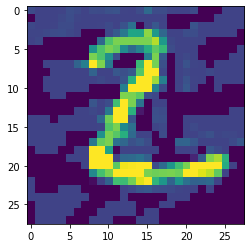
\includegraphics[width=\textwidth]{images/jpeg/fgsm_jpeg20_Le.png}
%     \caption{20\%}
% \end{subfigure}
% \hspace{1em}
% \begin{subfigure}[t]{0.22\textwidth}
% \centering
%     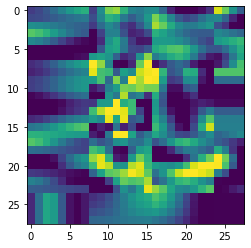
\includegraphics[width=\textwidth]{images/jpeg/fgsm_jpeg1_Le.png}
%     \caption{1\%}
% \end{subfigure}
% \caption{Ruido del ataque FGSM para distintas calidades en la compresión JPEG en el elemento \texttt{test[1]} de MNIST. En todos los casos, la red clasificó al 2 como un 7.}


% En la Figura \ref{Noise} se observa cómo el ruido generado por el ataque FGSM también se distorsiona conforme aumenta la compresión JPEG.



\subsection{Los efectos de Overfitting y Overparameterization}

Se ha sugerido que algunas propiedades de ciertas redes pueden contribuir a su suceptibilidad a los ataques adversarias. Por ejemplo, en el contexto de las imagenes médicas y sus redes respectivas, proponen que overfitting y overparameterization pueden actuar de esa manera \cite{ma2020understanding}. \textit{Overfitting} ocurre cuando el modelo clasifica bien los datos de entrenamiento, pero no se generaliza tan bien. Es decir, en los datos de validación, tiene peor desempeño. \textit{Overparameterization} tiene lugar cuando hay tantos parámetros que la red es capaz de ``memorizar'' completamente los datos. Hacemos un pequeño análisis para probar este hipótesis y no encontramos resultados que le apoyen. De hecho, con las redes que probamos, encontramos lo opuesto. En general, overfitting y overparameterization hacen que la red sea más robusto a los ataques adversarios (Figure \ref{overaparam_overfit}).

Para explorar lo de overfitting, cinco redes fueron entrenadas usado distintos numeros de épocas (epochs). Enre más épocas, más probabilidad de que la red haya sido overfit. Para ver lo mismo con overparameterization, seis redes fuernon entrenadas con distinas cantidades de parámetros. Se le metieron un cierto número de capas (layers) adicionales directamente antes de la última. Cada capa adicional tenía 256 nodos. Así que, probamos redes con varios números de parámetros (Cuadro \ref{overparam_table}).

\begin{table}[h]
    \centering
    \begin{tabular}{|c|c|}
     \hline
     Red & Número de parámetros  \\ 
     \hline
     Normal & $61,706$  \\ 
     \hline
     2 Capas Adicionales & $150,978$  \\ 
     \hline
     4 Capas Adicionales & $282,562$  \\ 
     \hline
     6 Capas Adicionales & $414,146$  \\ 
     \hline
     10 Capas Adicionales & $743,106$  \\ 
     \hline
     20 Capas Adicionales & $1,335,234$  \\ 
     \hline
    \end{tabular}
    \caption{table}
    \label{overparam_table}
\end{table}

\begin{figure}[h]
    \centering
    \begin{subfigure}[b]{0.49\textwidth}
        \centering
        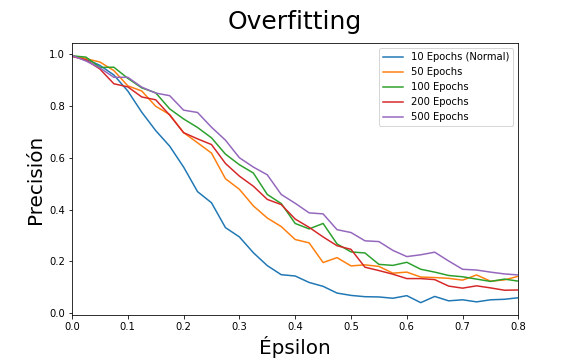
\includegraphics[width=\textwidth]{images/overfit_vs_attack.png}
        \caption{}
        \label{overfit}
    \end{subfigure}
    \begin{subfigure}[b]{0.49\textwidth}
        \centering
        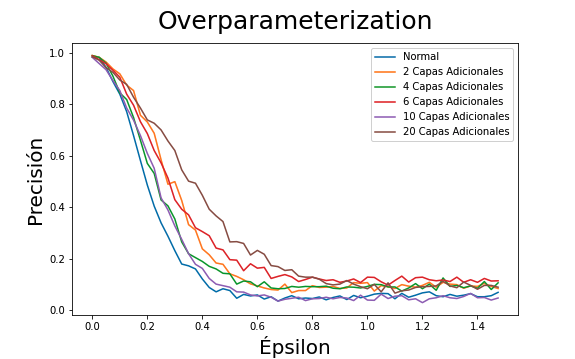
\includegraphics[width=\textwidth]{images/overparam_vs_attack.png}
        \caption{}
        \label{overparam}
    \end{subfigure}
    \caption{En (\ref{overfit}) se observa que conforme aumentamos el número de épocas (epochs), la precisión (accuracy) aumenta con respecto a cada épsilon. Asimismo en (\ref{overparam}), en general, aumentar el número de capas (layers) aumenta la precisión}
    \label{overaparam_overfit}
\end{figure}

\pagebreak
    
\subsection{Saliency}
\begin{itemize}
    \item Show figures from notebook of how adversarial noise attacks parts of the image that seem vulnerable (for example changing a 3$\to$8)
    \item Show Gradient-based localization of both image sets and how they change after adding adversarial noise\cite{Selvaraju_2019}
\end{itemize}




\pagebreak
\printbibliography





\end{document}


